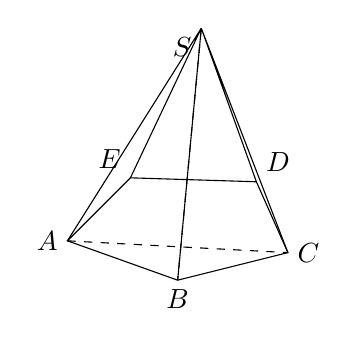
\begin{tikzpicture}[scale=1.0]
  \coordinate (S) at (0.4,2.5);
  \coordinate (A) at (-1.3,-0.2);
  \coordinate (B) at (0.1,-0.7);
  \coordinate (C) at (1.5,-0.35);
  \coordinate (D) at (1.1,0.55);
  \coordinate (E) at (-0.5,0.6);
  \draw (S) -- (A) (S) -- (B) (S) -- (C) (S) -- (D) (S) -- (E);
  \draw (A) -- (B) -- (C) -- (D) -- (E) -- cycle;
  \draw[dashed] (S) -- (B);
  \draw[dashed] (A) -- (C);
  \node[below left] at (S) {$S$};
  \node[left] at (A) {$A$};
  \node[below] at (B) {$B$};
  \node[right] at (C) {$C$};
  \node[above right] at (D) {$D$};
  \node[above left] at (E) {$E$};
\end{tikzpicture}
